\begin{figure}[t!]
    \centering
    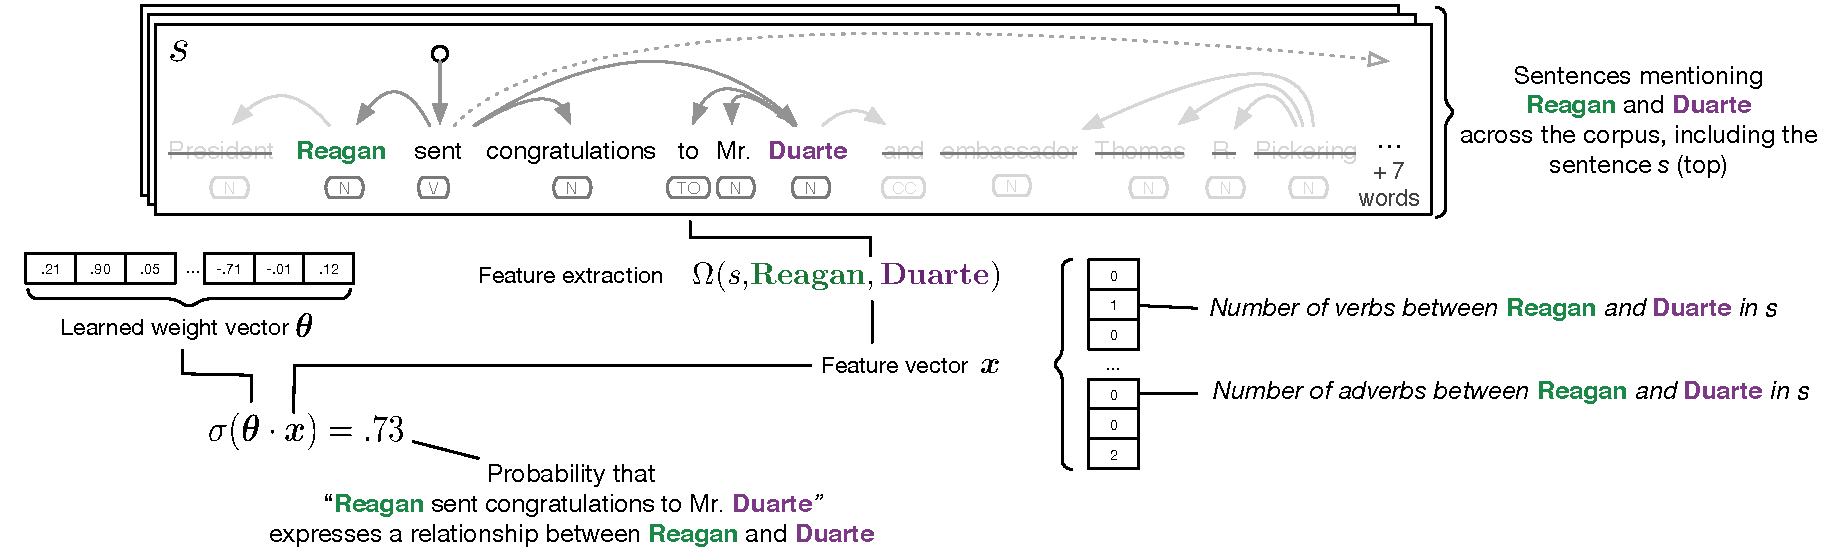
\includegraphics[width=.9\textwidth]{figures/rsum/rsum_big.pdf}
    \caption[Sentence simplification via relationship span extraction]{Sentence simplification via relationship span extraction \cite{handler-oconnor-2018-relational}.
    This method predicts the probability that the span of tokens between the query and subquery words in a given sentence $s$ will sound natural as a shorter and standalone sentence.
    (If the predicted probability is high, the sentence can likely be shortened to the span of tokens.)
    This figure shows the predicted probability that the token span between the query \textbf{\color{CCPurple}{Duarte}} and the subquery \textbf{\color{darkgreen}{Reagan}} will sound natural as a shortened sentence when extracted from the longer sentence shown in Figure \ref{f:system_cc} (letter K).
    Seven words from $s$ are not shown in the diagram above.}\label{f:rsum}
\end{figure}


% {\color[rgb]{0.000000,0.000000,0.000000}\Omega(s,} {\color[rgb]{.106, .471, .216}\text{\textbf{Reagan}}}, {\color[rgb]{.405, .144, .450}\text{\textbf{Duarte}}}{\color[rgb]{0.000000,0.000000,0.000000})}=\boldsymbol{x}_i 
